\documentclass[conference]{IEEEtran}
% Compiles with pdfLaTeX + BibTeX (Overleaf default) and with XeTeX (tectonic); Turkish letters
% outside Latin-1 are written as LaTeX accent commands so that both engines print them. Numbers and result tables are generated by
% tools/build_paper.py into generated/; do not type results by hand.
\usepackage[T1]{fontenc}
\usepackage[utf8]{inputenc}
\usepackage{cite}
\usepackage{amsmath,amssymb}
\usepackage{graphicx}
\usepackage{booktabs}
\usepackage{array}
\usepackage{adjustbox}
\usepackage{xspace}
\xspaceaddexceptions{\, \% ]}
\usepackage[hyphens]{url}
\usepackage{textcomp}
% generated by tools/build_paper.py - do not edit
\newcommand{\vRawRows}{3,938,630\xspace}
\newcommand{\vCellsDefined}{193\xspace}
\newcommand{\vCellsData}{156\xspace}
\newcommand{\vCellsKept}{153\xspace}
\newcommand{\vPctMissing}{6.5\xspace}
\newcommand{\vPctOutlier}{3.52\xspace}
\newcommand{\vNInvalid}{387\xspace}
\newcommand{\vNOutage}{1,387\xspace}
\newcommand{\vPanelRows}{4,077,120\xspace}
\newcommand{\vInvFiles}{61\xspace}
\newcommand{\vStudyMonths}{37\xspace}
\newcommand{\vFixtureRows}{310\xspace}
\newcommand{\vMatchesTotal}{263\xspace}
\newcommand{\vMatchesMain}{194\xspace}
\newcommand{\vMatchesValid}{176\xspace}
\newcommand{\vMatchesClosed}{69\xspace}
\newcommand{\vPctRelaxed}{41.8\xspace}
\newcommand{\vMeanControls}{2.7\xspace}
\newcommand{\vPreDS}{\ensuremath{-}2.86\xspace}
\newcommand{\vDuringDS}{\ensuremath{-}3.34\xspace}
\newcommand{\vPostDS}{\ensuremath{-}5.84\xspace}
\newcommand{\vPostPct}{\ensuremath{-}15.2\xspace}
\newcommand{\vPostDV}{14.7\xspace}
\newcommand{\vPostMedian}{\ensuremath{-}4.67\xspace}
\newcommand{\vPostSkew}{\ensuremath{-}1.37\xspace}
\newcommand{\vRingZero}{\ensuremath{-}9.44\xspace}
\newcommand{\vRingOne}{\ensuremath{-}5.32\xspace}
\newcommand{\vRingTwo}{\ensuremath{-}2.46\xspace}
\newcommand{\vDiD}{\ensuremath{-}5.12\xspace}
\newcommand{\vPlacebo}{\ensuremath{-}0.23\xspace}
\newcommand{\vPlaceboP}{0.189\xspace}
\newcommand{\vClosedDoors}{0.16\xspace}
\newcommand{\vClosedDoorsP}{0.648\xspace}
\newcommand{\vQCPassed}{14/14\xspace}
\newcommand{\vShapiroShare}{33\xspace}
\newcommand{\vPostCI}{[\ensuremath{-}6.45, \ensuremath{-}5.22]\xspace}
\newcommand{\vPostRams}{\ensuremath{-}9.54\xspace}
\newcommand{\vPostSaracoglu}{\ensuremath{-}4.41\xspace}
\newcommand{\vPostTupras}{\ensuremath{-}3.11\xspace}
\newcommand{\vHTwoTests}{23\xspace}
\newcommand{\vHTwoSigRaw}{7\xspace}
\newcommand{\vHTwoSigHolm}{5\xspace}
\newcommand{\vHTwoSigRawParam}{8\xspace}
\newcommand{\vHTwoSigHolmParam}{6\xspace}
\newcommand{\vHOneTests}{36\xspace}
\newcommand{\vHOneSigHolm}{32\xspace}
\newcommand{\vHOneSpeedSigHolm}{9\xspace}
\newcommand{\vBigMean}{\ensuremath{-}7.64\xspace}
\newcommand{\vBigOther}{\ensuremath{-}5.62\xspace}
\newcommand{\vBigN}{18\xspace}
\newcommand{\vBigP}{0.047\xspace}
\newcommand{\vBigPU}{0.209\xspace}
\newcommand{\vBigPHolm}{0.746\xspace}
\newcommand{\vIstMean}{\ensuremath{-}5.60\xspace}
\newcommand{\vIstOther}{\ensuremath{-}5.72\xspace}
\newcommand{\vIstP}{0.886\xspace}
\newcommand{\vOppAnovaP}{0.255\xspace}
\newcommand{\vOppKwP}{0.657\xspace}
\newcommand{\vOppEta}{0.024\xspace}
\newcommand{\vStEta}{0.47\xspace}
\newcommand{\vCompKwP}{0.004\xspace}
\newcommand{\vCompKwPHolm}{0.073\xspace}
\newcommand{\vChiSq}{847\xspace}
\newcommand{\vCramerV}{0.073\xspace}
\newcommand{\vChiN}{159,232\xspace}
\newcommand{\vCongWin}{25.2\xspace}
\newcommand{\vCongOther}{18.3\xspace}
\newcommand{\vSensN}{110\xspace}
\newcommand{\vSensMean}{\ensuremath{-}5.88\xspace}
\newcommand{\vSensCI}{[\ensuremath{-}6.66, \ensuremath{-}5.09]\xspace}
\newcommand{\vCells}{65\xspace}
\newcommand{\vTestMatches}{44\xspace}
\newcommand{\vNFeatures}{41\xspace}
\newcommand{\vTrainRows}{908,237\xspace}
\newcommand{\vTestRows}{267,248\xspace}
\newcommand{\vTestMatchRows}{7,138\xspace}
\newcommand{\vSelTrainRows}{474,280\xspace}
\newcommand{\vSelValRows}{433,908\xspace}
\newcommand{\vTrainFree}{51.4\xspace}
\newcommand{\vTestFree}{49.1\xspace}
\newcommand{\vTrainModerate}{40.8\xspace}
\newcommand{\vTestModerate}{42.8\xspace}
\newcommand{\vTrainCongested}{7.8\xspace}
\newcommand{\vTestCongested}{8.1\xspace}
\newcommand{\vTThreePrevTrain}{2.4\xspace}
\newcommand{\vTThreePrevTest}{3.1\xspace}
\newcommand{\vTThreePrevSelTrain}{2.3\xspace}
\newcommand{\vTThreePrevSelVal}{5.9\xspace}
\newcommand{\vBestLeaves}{31\xspace}
\newcommand{\vBestCW}{none\xspace}
\newcommand{\vFOneHgbAll}{0.797\xspace}
\newcommand{\vFOneHgbMatch}{0.702\xspace}
\newcommand{\vFCongHgbPost}{0.533\xspace}
\newcommand{\vMaeHgbAll}{2.38\xspace}
\newcommand{\vMaeHgbMatch}{3.12\xspace}
\newcommand{\vMaeHgbPost}{3.68\xspace}
\newcommand{\vFOneNoEvAll}{0.794\xspace}
\newcommand{\vFOneNoEvMatch}{0.633\xspace}
\newcommand{\vFCongNoEvPost}{0.038\xspace}
\newcommand{\vMaeNoEvAll}{2.41\xspace}
\newcommand{\vMaeNoEvMatch}{4.07\xspace}
\newcommand{\vMaeNoEvPost}{6.68\xspace}
\newcommand{\vFOneRfAll}{0.779\xspace}
\newcommand{\vFOneRfMatch}{0.663\xspace}
\newcommand{\vFCongRfPost}{0.510\xspace}
\newcommand{\vMaeRfAll}{2.46\xspace}
\newcommand{\vMaeRfMatch}{3.64\xspace}
\newcommand{\vMaeRfPost}{5.44\xspace}
\newcommand{\vFOneLinAll}{0.751\xspace}
\newcommand{\vFOneLinMatch}{0.597\xspace}
\newcommand{\vFCongLinPost}{0.555\xspace}
\newcommand{\vMaeLinAll}{2.60\xspace}
\newcommand{\vMaeLinMatch}{3.97\xspace}
\newcommand{\vMaeLinPost}{5.25\xspace}
\newcommand{\vFOneBZeroAll}{0.742\xspace}
\newcommand{\vFOneBZeroMatch}{0.613\xspace}
\newcommand{\vFCongBZeroPost}{0.133\xspace}
\newcommand{\vMaeBZeroAll}{3.09\xspace}
\newcommand{\vMaeBZeroMatch}{4.74\xspace}
\newcommand{\vMaeBZeroPost}{7.18\xspace}
\newcommand{\vFOneBOneAll}{0.746\xspace}
\newcommand{\vFOneBOneMatch}{0.607\xspace}
\newcommand{\vFCongBOnePost}{0.064\xspace}
\newcommand{\vMaeBOneAll}{2.84\xspace}
\newcommand{\vMaeBOneMatch}{4.31\xspace}
\newcommand{\vMaeBOnePost}{6.80\xspace}
\newcommand{\vPrHgbAll}{0.147\xspace}
\newcommand{\vPrHgbMatch}{0.501\xspace}
\newcommand{\vPrNoEvAll}{0.088\xspace}
\newcommand{\vPrNoEvMatch}{0.196\xspace}
\newcommand{\vPrLinAll}{0.105\xspace}
\newcommand{\vPrLinMatch}{0.280\xspace}
\newcommand{\vPrBZeroAll}{0.072\xspace}
\newcommand{\vPrBZeroMatch}{0.142\xspace}
\newcommand{\vMaeGainPost}{45\xspace}
\newcommand{\vRTwoHgbAll}{0.944\xspace}
\newcommand{\vImpHistoryAll}{0.458\xspace}
\newcommand{\vImpHistoryMatch}{0.343\xspace}
\newcommand{\vImpEventAll}{0.005\xspace}
\newcommand{\vImpEventMatch}{0.070\xspace}
\newcommand{\vImpSpatialAll}{0.025\xspace}
\newcommand{\vImpSpatialMatch}{0.064\xspace}
\newcommand{\vImpCalendarAll}{0.014\xspace}
\newcommand{\vImpCalendarMatch}{0.005\xspace}
\newcommand{\vImpWeatherAll}{0.001\xspace}
\newcommand{\vImpWeatherMatch}{\ensuremath{-}0.001\xspace}
\newcommand{\vCongRecall}{51\xspace}
\newcommand{\vCongAsModerate}{45\xspace}
\newcommand{\vFreeRecall}{78\xspace}
\newcommand{\vModRecall}{78\xspace}
\newcommand{\vPostCongObs}{14.9\xspace}
\newcommand{\vPostCongHgb}{9.8\xspace}
\newcommand{\vPostCongNoEv}{1.1\xspace}
\newcommand{\vPeakObs}{26.0\xspace}
\newcommand{\vPeakHgb}{27.0\xspace}
\newcommand{\vPeakNoEv}{36.2\xspace}
\newcommand{\vBrierHgb}{0.0283\xspace}
\newcommand{\vBrierRef}{0.0300\xspace}
\newcommand{\vBrierNoEv}{0.0294\xspace}
\newcommand{\vBrierLin}{0.2263\xspace}
\newcommand{\vTThreeMeanPred}{2.5\xspace}
\newcommand{\vLogLossTTwo}{0.360\xspace}
\newcommand{\vBrierTTwo}{0.214\xspace}
\newcommand{\vBrierTTwoRef}{0.569\xspace}
\newcommand{\vBootMatches}{43\xspace}
\newcommand{\vBootMae}{0.96\xspace}
\newcommand{\vBootMaeCI}{[0.69, 1.23]\xspace}
\newcommand{\vBootFOne}{0.068\xspace}
\newcommand{\vBootFOneCI}{[0.050, 0.089]\xspace}
\newcommand{\vExtRailFirst}{January 2021\xspace}
\newcommand{\vExtRailLast}{December 2025\xspace}
\newcommand{\vExtRailN}{268\xspace}
\newcommand{\vExtRailMean}{81\xspace}
\newcommand{\vExtRailMedian}{40\xspace}
\newcommand{\vExtRailCI}{[70, 93]\xspace}
\newcommand{\vExtRailRams}{181\xspace}
\newcommand{\vExtRailRamsMed}{139\xspace}
\newcommand{\vExtRailSar}{32\xspace}
\newcommand{\vExtRailSarMed}{32\xspace}
\newcommand{\vExtRailTup}{31\xspace}
\newcommand{\vExtRailTupMed}{26\xspace}
\newcommand{\vExtRailStudy}{83\xspace}
\newcommand{\vExtRailStudyN}{199\xspace}
\newcommand{\vExtRailAfter}{76\xspace}
\newcommand{\vExtRailAfterN}{69\xspace}
\newcommand{\vExtRailAfterCI}{[53, 98]\xspace}
\newcommand{\vExtRailAfterMed}{38\xspace}
\newcommand{\vExtRailClosed}{\ensuremath{-}13\xspace}
\newcommand{\vExtRailClosedMed}{\ensuremath{-}2\xspace}
\newcommand{\vExtRailClosedN}{42\xspace}
\newcommand{\vExtRailClosedP}{0.084\xspace}
\newcommand{\vExtLinkRho}{\ensuremath{-}0.59\xspace}
\newcommand{\vExtLinkN}{170\xspace}
\newcommand{\vExtDerby}{121\xspace}
\newcommand{\vExtNonDerby}{78\xspace}
\newcommand{\vExtDerbyP}{0.127\xspace}
\newcommand{\vExtUymRows}{148,530\xspace}
\newcommand{\vExtUymLast}{31 October 2026\xspace}
\newcommand{\vExtUymFootball}{296\xspace}
\newcommand{\vExtUymWith}{249\xspace}
\newcommand{\vExtUymMatches}{329\xspace}
\newcommand{\vExtUymShare}{76\xspace}
\newcommand{\vExtUymClosure}{40\xspace}
\newcommand{\vExtUymBefore}{99\xspace}
\newcommand{\vExtUymMedianH}{4.0\xspace}
\newcommand{\vExtUymAfterWith}{118\xspace}
\newcommand{\vExtUymClosedWith}{0\xspace}
\newcommand{\vExtUymClosedMatches}{69\xspace}
\newcommand{\vExtIncRR}{1.16\xspace}
\newcommand{\vExtIncCI}{[0.80, 1.61]\xspace}
\newcommand{\vExtFixAfter}{137\xspace}


\newcommand{\fitcol}[1]{\begin{adjustbox}{max width=\columnwidth}#1\end{adjustbox}}

\begin{document}

\title{Do Football Matches Slow Down Istanbul?\\Measuring and Predicting Match-Day Traffic\\around Three Stadiums with Open Data}

\author{
\IEEEauthorblockN{Mustafa Eren Atasoy}
\IEEEauthorblockA{Dept. of Computer Engineering\\
\.{I}stanbul Kültür University\\
\.{I}stanbul, Türkiye\\
Student ID 2200003501}
\and
\IEEEauthorblockN{Ka\u{g}an Kutano\u{g}lu}
\IEEEauthorblockA{Dept. of Computer Engineering\\
\.{I}stanbul Kültür University\\
\.{I}stanbul, Türkiye\\
Student ID 2300006719}
\and
\IEEEauthorblockN{Ahmet Recep Özdemir}
\IEEEauthorblockA{Dept. of Computer Engineering\\
\.{I}stanbul Kültür University\\
\.{I}stanbul, Türkiye\\
Student ID 2200003305}
}

\maketitle

\begin{abstract}
Rams Park, \c{S}ükrü Saraco\u{g}lu Stadium and Tüpra\c{s} Stadyumu each hold more than 40,000 spectators and lie in congested parts of Istanbul. We ask whether matches at these venues change local traffic and whether the change can be predicted a day in advance. Hourly speeds and observed-vehicle counts of the Istanbul Metropolitan Municipality, published per 6-character geohash cell, were combined with official fixtures, ERA5 weather and the holiday calendar for three seasons with spectators and one closed-doors placebo season. Each match was compared with up to four matched control days, and inference was made with one observation per match. In the three hours after the final whistle, average speed in the stadium cell and its neighbours changes by \vPostDS km/h (\vPostPct\,\%) relative to the control days (Wilcoxon $p<0.001$); the effect is largest at Rams Park (\vPostRams km/h), weakens with distance, survives Holm correction and is absent on placebo dates and in the closed-doors season. Its size depends on the stadium but not on derby status, opponent, kick-off time or weather. For prediction, a day-ahead, leakage-controlled setting was used with forward-chaining validation and a single test on the 2024-25 season. Histogram gradient boosting reached a macro-F1 of \vFOneHgbAll for a three-class congestion target, ahead of logistic regression, a random forest and two seasonal baselines. Fixture features barely matter over all hours, but in the post-match hours near the stadiums they cut the speed error from \vMaeNoEvPost to \vMaeHgbPost km/h, by \vMaeGainPost\,\%; a bootstrap over matches confirms the gain. Two further open sources, daily entries at the rail stations next to the stadiums and the announcements of the municipal traffic control centre, confirm the crowd effect independently and show that it continues after the traffic data end in January 2025.
\end{abstract}

\begin{IEEEkeywords}
traffic prediction, planned special events, football, geohash, hypothesis testing, gradient boosting, data leakage, Istanbul
\end{IEEEkeywords}

% =====================================================================
\section{Introduction}
Istanbul is one of the most congested cities in the world; the 2024 INRIX scorecard ranked it first among 946 urban areas \cite{inrix}. Its three largest club stadiums sit in very different but equally sensitive parts of this network: Tüpra\c{s} Stadyumu on the Bosphorus shore road in Be\c{s}ikta\c{s}, \c{S}ükrü Saraco\u{g}lu Stadium inside the dense fabric of Kad{\i}köy, and Rams Park in Seyrantepe on the European side. A planned special event adds a concentrated and scheduled travel demand to a network that may already be close to capacity \cite{fhwa2003}. Whether this produces measurable slowdowns, where and for how long is not obvious: many fans use public transport, background traffic may avoid the area, police close streets, and the event demand may coincide with, or replace, the evening peak.

Because fixtures are published weeks in advance, match-day disruptions are among the most predictable irregularities of urban traffic. Knowing their size helps traffic managers time closures and signal plans, helps public-transport operators plan extra services, and helps residents plan their trips. We study three research questions:
\begin{itemize}
\item \textbf{RQ1} Do matches cause statistically significant changes in speed and in the number of observed vehicles around the stadiums before, during and after the match?
\item \textbf{RQ2} Do the effects differ by stadium, kick-off time, derby status, opponent, competition, weekday or weather?
\item \textbf{RQ3} Can congestion around the stadiums be predicted one day ahead, and does fixture information improve that prediction?
\end{itemize}
Each question is tested through falsifiable hypotheses. \textbf{H1}: the mean match-minus-control change in speed is zero in every window. \textbf{H2}: the post-match change does not differ between groups of matches. \textbf{H3}: the change is equal in the stadium cell and in the surrounding rings. \textbf{H4}: pseudo-events and closed-doors matches show no change. \textbf{H5}: adding fixture features does not reduce the day-ahead prediction error in match windows.

Our contributions are (i) a reproducible open-data pipeline that turns the municipal traffic files into an analysis-ready cell-hour dataset with documented quality checks, (ii) a matched control-day design with placebo, closed-doors, difference-in-differences and spatial-decay checks, (iii) a leakage-controlled day-ahead prediction study that compares four model families against seasonal baselines and isolates the value of fixture information, and (iv) evidence on the size, timing and location of match-day slowdowns in Istanbul.

% =====================================================================
\section{Literature Review}
\textit{Operational guidance.} The U.S. Federal Highway Administration handbook \cite{fhwa2003} treats stadium events as scheduled demand that can be planned for, but gives no empirical estimate of their impact.

\textit{Econometric evidence.} Humphreys and Pyun \cite{humphreys2018} used instrumental-variable regression on 25 U.S. metropolitan areas and found that Major League Baseball attendance increases vehicle-miles travelled and traffic delay. Hwang \textit{et al.} \cite{hwang2025} analysed taxi trips around Yankee Stadium and reported about 1.3\,\% longer travel times on game days, with larger effects for trips through the stadium area. Giuliano and Lu \cite{giuliano2021} compared game days with control days at the Los Angeles Memorial Coliseum using detector speeds on highways and arterials and found that a random forest outperformed a regression model. Pulugurtha \textit{et al.} \cite{pulugurtha2020} examined how travel-time measures change over time and with distance from two planned events.

\textit{Prediction with event information.} Kwoczek \textit{et al.} proposed approaches to predict congestion in the presence of planned events \cite{kwoczek2014} and to identify the road segments affected around stadiums \cite{kwoczek2015}. Rodrigues \textit{et al.} \cite{rodrigues2019} showed that adding event information mined from the web to time-series models reduces taxi-demand forecasting errors in event areas of New York.

\textit{Istanbul.} The municipal hourly traffic data have recently been used by \c{S}ahin and Çolako\u{g}lu \cite{sahin2025}, who analysed one month of a single Be\c{s}ikta\c{s} coastal cell with SARIMA and random forest models; this cell (\texttt{sxk9kp}) belongs to the first ring of Tüpra\c{s} Stadyumu in our design. Özdenizci Köse \textit{et al.} \cite{ozdenizci2025} related Istanbul traffic density to meteorological and temporal variables and compared regression, ensemble and neural-network models. Olug \textit{et al.} \cite{olug2024} released a graph benchmark of 2,451 Istanbul sensor locations.

\textit{Gap.} Existing event studies are U.S.-based and use proprietary detector, probe or taxi data; they analyse few venues, often compare match days with ``average'' days, and treat correlated hours as independent observations. The Istanbul studies explain traffic with calendar and weather variables only. No study has measured football effects in Istanbul, combined a falsifiable counterfactual design with day-ahead prediction, or quantified what fixture information adds to a leakage-free forecast. Table~\ref{tab:lit} summarises the comparison.

\begin{table*}[t]
\caption{Comparison of related studies with this work}
\label{tab:lit}
\centering\footnotesize
\begin{tabular}{@{}>{\raggedright\arraybackslash}p{2.5cm}>{\raggedright\arraybackslash}p{3.5cm}>{\raggedright\arraybackslash}p{3.5cm}>{\raggedright\arraybackslash}p{3.3cm}>{\raggedright\arraybackslash}p{3.5cm}@{}}
\toprule
Study & Data & Setting / unit & Counterfactual & Methods \\
\midrule
Humphreys \& Pyun \cite{humphreys2018} & Urban mobility statistics & 25 U.S. metro areas, 1990--2014 & Variation across cities and years & Instrumental-variable regression \\
Hwang \textit{et al.} \cite{hwang2025} & Taxi trips & Yankee Stadium, New York & Game vs.\ non-game days & Econometric comparison \\
Giuliano \& Lu \cite{giuliano2021} & In-road detector speeds & LA Coliseum, highways and arterials & Game vs.\ control days & Regression, random forest \\
Rodrigues \textit{et al.} \cite{rodrigues2019} & Taxi demand + web event text & Event areas, New York & Forecasts without event data & Deep learning \\
\c{S}ahin \& Çolako\u{g}lu \cite{sahin2025} & IBB geohash vehicle counts & 1 cell, 1 month, hourly & Weekday vs.\ weekend & SARIMA, random forest \\
\textbf{This work} & IBB speeds and vehicles, TFF fixtures, ERA5 weather, holidays & 3 stadiums $\times$ geohash rings, 3.5 seasons, hourly & Matched control days, placebo dates, closed-doors season, distal-ring DiD & Match-level tests with Holm correction; day-ahead models with ablation \\
\bottomrule
\end{tabular}
\end{table*}

% =====================================================================
\section{Data}
\subsection{Sources}
\textit{Traffic.} The Hourly Traffic Density Data Set of the Istanbul Metropolitan Municipality (IBB) \cite{ibb_data} reports, for every 6-character geohash cell \cite{geohash} and hour, the minimum, maximum and average speed and the number of distinct observed vehicles. A cell spans about 0.61\,km $\times$ 0.92\,km and contains several road types, so all spatial variables are defined at cell or ring level. The vehicle count is a sample and is used only as a relative intensity indicator, never as traffic volume. The portal lists \vInvFiles monthly files (January 2020 to January 2025, no gaps; no later file had been published by November 2026); the \vStudyMonths study months contain \vRawRows records of the study cells, retrieved through the portal's CKAN API with a server-side cell filter.

\textit{Fixtures.} Home matches of Galatasaray, Fenerbahçe and Be\c{s}ikta\c{s} in the league and domestic cups were collected from the match pages of the Turkish Football Federation \cite{tff}; UEFA home matches, which the federation does not publish, were added from the clubs' English Wikipedia season articles \cite{wiki_seasons} with Turkey-time kick-offs. Of \vFixtureRows rows, neutral-venue finals, forfeited matches without a date, three UEFA matches without a stated time zone and matches outside the study periods were removed, leaving \vMatchesTotal matches (\vMatchesMain in the main seasons, \vMatchesClosed in the closed-doors season).

\textit{Weather and calendar.} Hourly ERA5 reanalysis \cite{era5} was retrieved for each stadium from the Open-Meteo archive \cite{openmeteo} in the Europe/Istanbul time zone. Public holidays, religious-holiday eves and the national mourning week after the February 2023 earthquakes were added as calendar information.

\textit{Additional sources (extension).} Because the traffic series ends in January 2025 and no other open source provides cell-level speeds for Istanbul, two further IBB data sets were added to validate the findings and to extend them in time: daily entries per rail station \cite{ibb_rail} (\vExtRailFirst to \vExtRailLast) and the announcements of the Transport Management Centre (UYM) with start time, type, title and coordinates \cite{ibb_uym} (\vExtUymRows announcements from July 2020 to \vExtUymLast). The stations next to the stadiums are Seyrantepe (M2, with a stadium exit) for Rams Park, Sö\u{g}ütlüçe\c{s}me (Marmaray, about 400\,m away) for \c{S}ükrü Saraco\u{g}lu and Kabata\c{s} (T1 and F1) for Tüpra\c{s}. Fixtures of the 2025-26 and 2026-27 seasons were collected from the same sources as before (\vExtFixAfter home matches after January 2025). These data are used only in Section~\ref{sec:external} and do not enter the main analysis.

\subsection{Seasons and spatial units}
The 2022-23 and 2023-24 seasons and the 2024-25 season up to January 2025 (the last published month) are the main seasons. The 2021-22 season was excluded because it began with attendance capped at 50\,\% \cite{karar2021}, and the 2020-21 season, played behind closed doors, serves as a placebo. Around each stadium, the cell containing the stadium is R0; the Chebyshev rings at distance 1 and 2 on the geohash grid form R1 (8 cells) and R2 (16 cells), and a distal ring at distance 5 (40 cells, 3--4.6\,km away) serves as a reference area (Fig.~\ref{fig:area}). R0 and R1 together form the NEAR ring, the main unit of the statistical analysis.

\begin{figure*}[t]
\centering
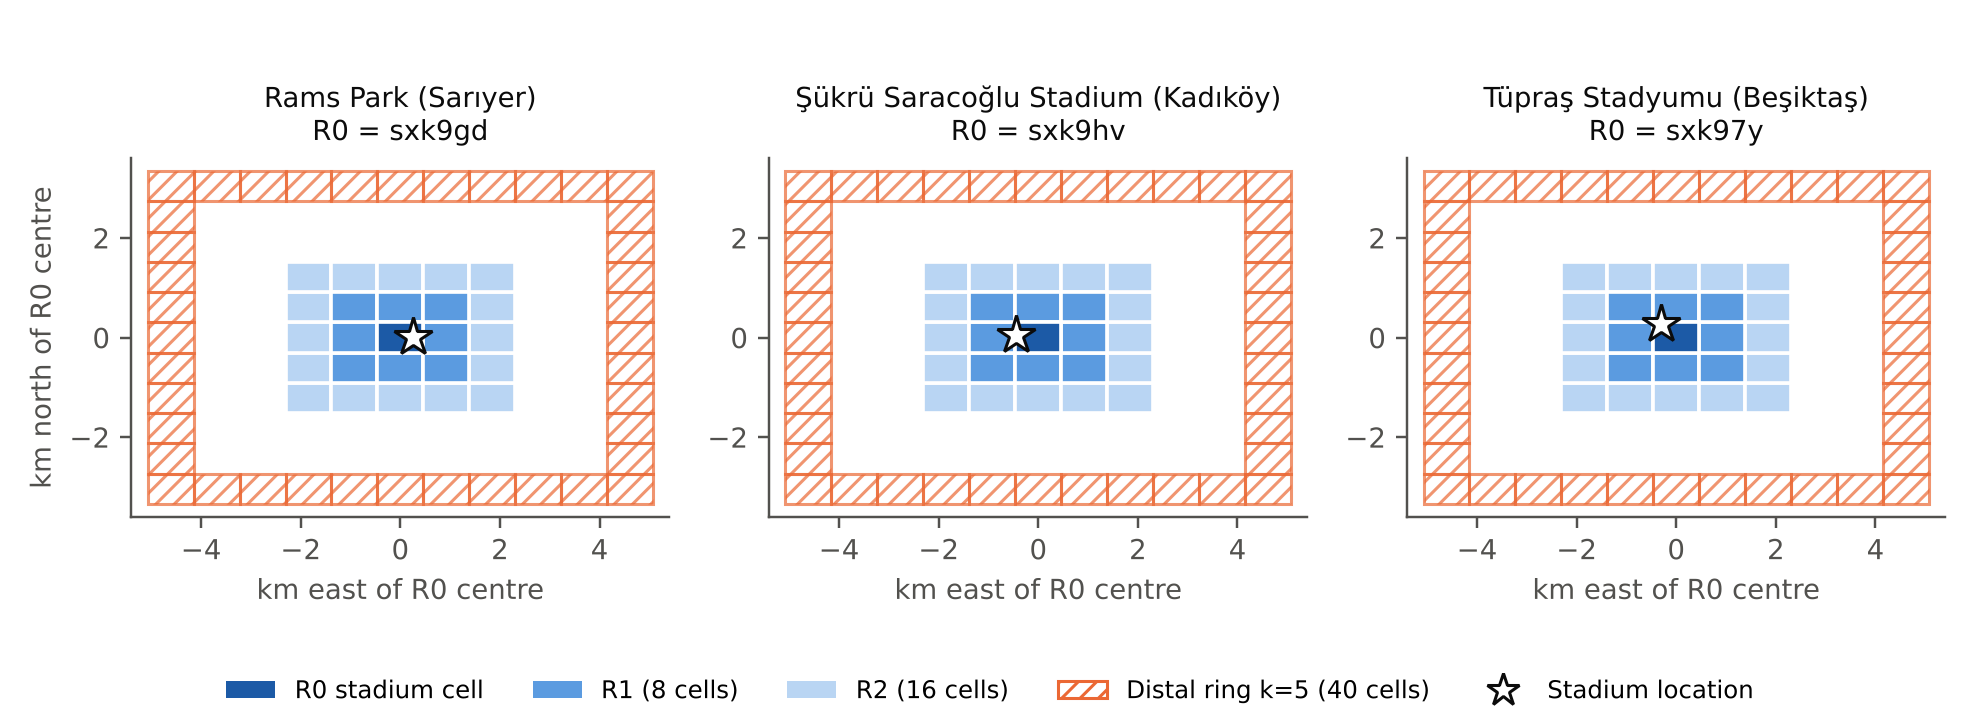
\includegraphics[width=0.78\textwidth]{figures/fig_3_1_study_area.png}
\caption{Geohash rings around the three stadiums (one cell $\approx$ 0.61\,km $\times$ 0.92\,km).}
\label{fig:area}
\end{figure*}

\subsection{Dataset statistics}
Of \vCellsDefined defined study cells, \vCellsData contain data and \vCellsKept have at least 80\,\% hourly coverage. The analysis-ready panel has \vPanelRows cell-hours; \vPctMissing\,\% of the cell-hours are missing (mostly system-wide outage hours) and \vPctOutlier\,\% are flagged as outliers. The modelling set contains the \vCells analysed cells of R0--R2 in the main seasons: \vTrainRows labelled cell-hours for training (2022-24) and \vTestRows for testing (2024-25), of which \vTestMatchRows fall in match windows. Each cell-hour has \vNFeatures features. The classes of the primary target are imbalanced: \vTrainFree\,\% free, \vTrainModerate\,\% moderate and \vTrainCongested\,\% congested hours in training (\vTestFree, \vTestModerate and \vTestCongested\,\% in the test season); the abnormal-slowdown event occurs in \vTThreePrevTrain\,\% of the training hours.

% =====================================================================
\section{Methodology}
Fig.~\ref{fig:workflow} summarises the workflow. All parameters are set in one configuration file, and one command rebuilds the dataset, every statistic, every model and the tables of this paper.

\begin{figure*}[t]
\centering
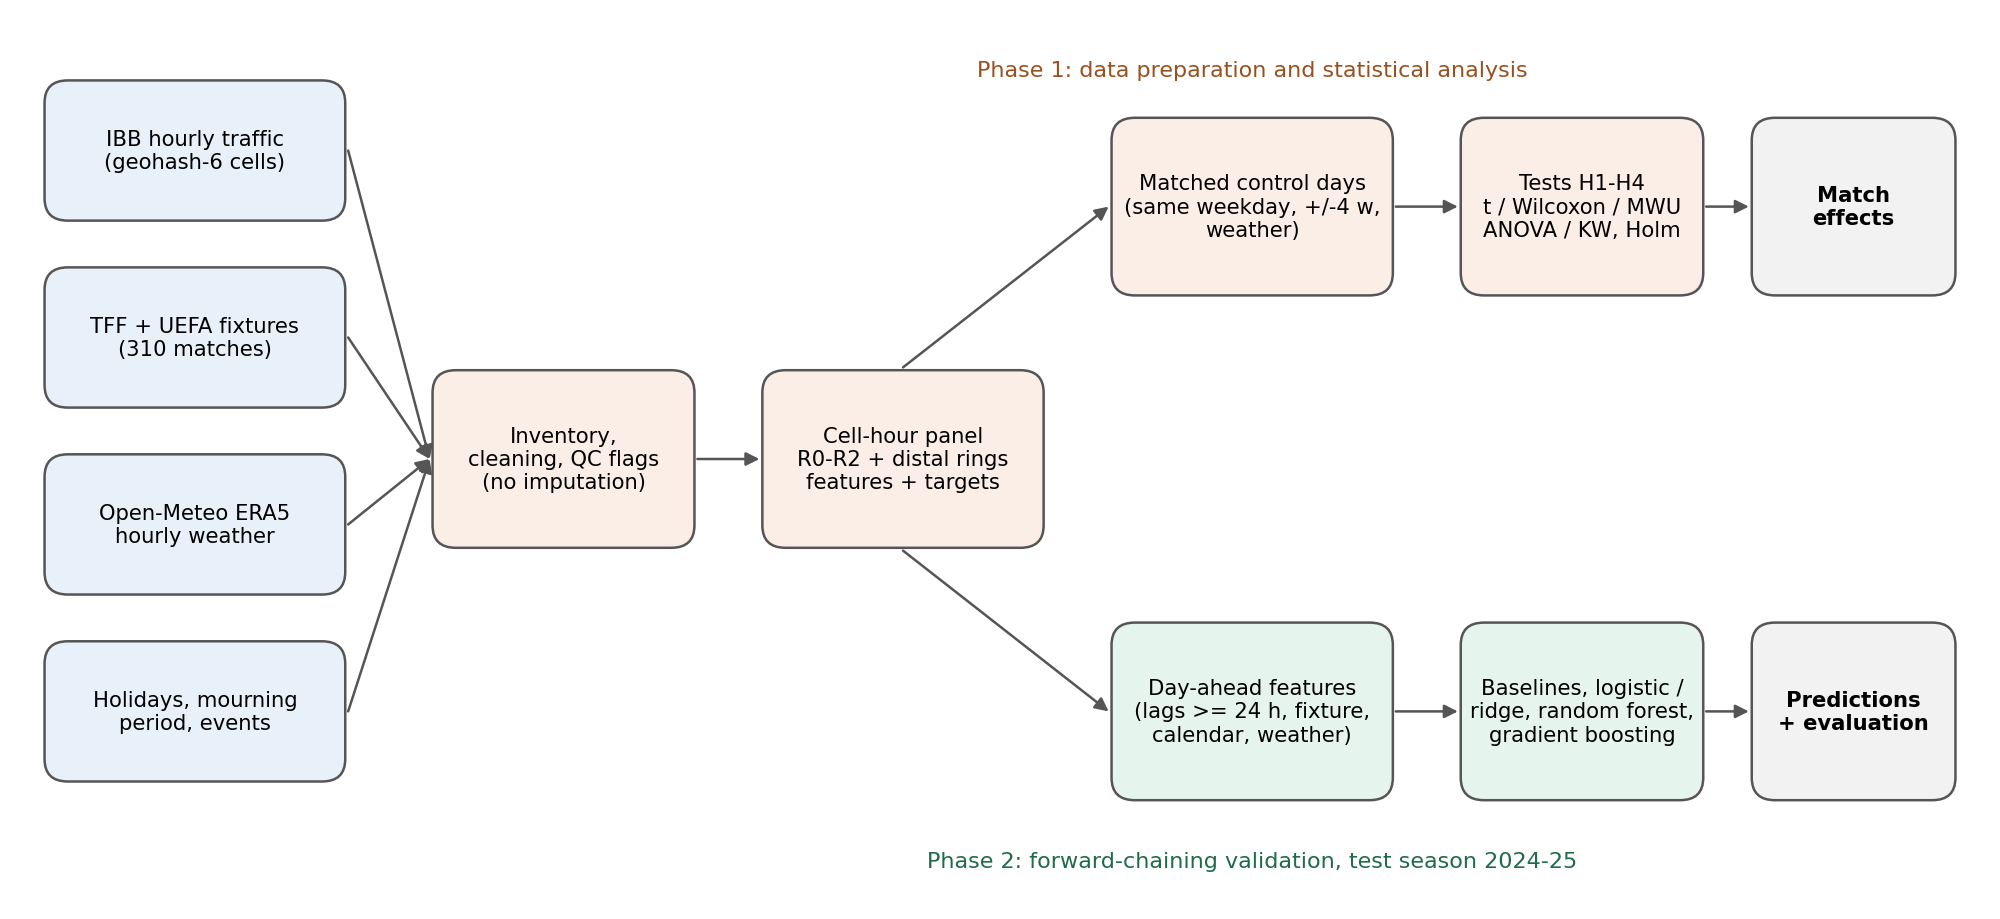
\includegraphics[width=0.82\textwidth]{figures/fig_workflow.png}
\caption{Workflow from the raw sources to the statistical and predictive results.}
\label{fig:workflow}
\end{figure*}

\subsection{Preprocessing and feature engineering}
Time stamps were parsed (the portal uses two formats) and localised to Europe/Istanbul; the local-time assumption was verified because the hour with the fewest vehicles is 03:00. Exact duplicates were removed and repeated cell-hour keys aggregated; speeds outside 0--200\,km/h, rows violating minimum\,$\le$\,average\,$\le$\,maximum and zero-vehicle rows were set to missing (\vNInvalid values). Every cell was reindexed to a complete hourly grid, and hours in which more than half of the cells were missing were flagged as outages (\vNOutage hours). Missing values were \emph{not} imputed, because an imputed value inside a match window would be an artificial observation. Outliers were detected with the interquartile-range rule \cite{tukey1977} within each cell and hour of the week and flagged rather than removed, because a match-day slowdown is by definition an unusual value. Cells below 80\,\% coverage and hours with fewer than five observed vehicles (unreliable speeds) were excluded from the analyses. Feature engineering followed the course procedures: a log transform of vehicle counts, z-score standardisation and min--max normalisation within each cell, equal-width and equal-frequency discretisation, dummy variables for the event window and cyclic (sine/cosine) encoding of the hour. Fourteen automated quality checks run at the end of every build (\vQCPassed passed).

\subsection{Control days and effect measure}
Kick-off is rounded to the nearest hour (KO) and three windows are analysed: \emph{pre} ($-3$ to $-1$\,h), \emph{during} (0 to $+1$\,h) and \emph{post} ($+2$ to $+4$\,h). For each match, candidate control days are the same weekday one to four weeks before or after. A candidate is rejected if any of the three stadiums hosts a match on that day or the day before, if it is a holiday, a holiday eve or in the mourning week, if fewer than 80\,\% of its hours are observed, or if its weather differs (more than 5\,$^\circ$C at KO or a different wet/dry state). The four nearest valid days are kept; when fewer than two pass the weather rule it is relaxed and the match is flagged. For match $m$, ring $r$ and relative hour $h$ the effect is
\begin{equation}
\Delta_{m,r,h} = y_{m,r,h} - \frac{1}{|C_m|}\sum_{c\in C_m} y_{c,r,h},
\label{eq:delta}
\end{equation}
where $C_m$ is the set of control days and $y$ is the ring mean of speed or of $\log(1+\text{vehicles})$. Window effects are averages of \eqref{eq:delta} over the hours of a window, which gives exactly one value per match, ring and window. Using one value per match avoids pseudo-replication: neighbouring hours and cells of one match are strongly correlated.

\subsection{Statistical analysis}
For H1, the normality of the per-match differences was checked with the Shapiro--Wilk test \cite{shapiro1965}; the paired t-test and the Wilcoxon signed-rank test \cite{wilcoxon1945} were both reported, with the rank test as the main test when normality was rejected. For H2, pairs of groups were compared with the Levene test \cite{levene1960}, Student's or Welch's t-test \cite{welch1947} and the Mann--Whitney U test \cite{mann1947}; factors with three or more groups (stadium, competition, kick-off slot and opponent group) were tested with one-way ANOVA and the Kruskal--Wallis test \cite{kruskal1952}, with $\eta^2$ as the effect size. Opponents were grouped into big matches (derby or Trabzonspor), other Istanbul clubs (few travelling fans), other domestic clubs and European clubs. Pearson, Spearman and Kendall correlations related the effect to match attributes. H3 compared neighbouring rings with paired tests, and H4 used pseudo-events placed on non-match days, the closed-doors season and a difference-in-differences against the distal ring. Because many tests were run, Holm's step-down procedure \cite{holm1979} was applied within each hypothesis family. A sensitivity analysis repeated H1 without the matches whose weather rule was relaxed, and a chi-square test with Cramér's $V$ \cite{cramer1946} related the congestion class to the match window. All tests use $\alpha=0.05$ and SciPy \cite{scipy}.

\subsection{Prediction task and leakage control}
The unit of prediction is one cell-hour in the analysed R0--R2 cells, and the horizon is one day: a traffic operator wants to know today what will happen at each hour tomorrow. A feature is therefore admissible only if it is known at least 24 hours before the target hour (Table~\ref{tab:features}). Same-hour traffic values, and features derived from them such as the per-cell z-scores of Phase 1, are excluded because they contain the answer \cite{kaufman2012}. The quantities that define the targets---the free-flow speed of each cell and the hour-of-week mean and standard deviation---are recomputed on the training period only. Historical ERA5 weather stands in for a weather forecast; this is optimistic but has little influence, as Section~\ref{sec:importance} shows.

\begin{table}[t]
\caption{Feature groups of the day-ahead models (\vNFeatures features)}
\label{tab:features}
\centering\footnotesize
\begin{tabular}{@{}p{1.35cm}p{6.6cm}@{}}
\toprule
Group & Features \\
\midrule
History & speed 24, 48 and 168\,h earlier; mean of the same hour in the previous four weeks; log vehicles 24 and 168\,h earlier; the same lags as ratios to the free-flow speed; hour-of-week mean speed and ratio of the training period \\
Event & match day at this stadium; match at any of the three stadiums; hour relative to kick-off; competition; kick-off slot; derby; big match; opponent group; capacity \\
Calendar & hour (also as sine/cosine), weekday, month, weekend, holiday, holiday eve \\
Weather & temperature, precipitation, rain, snowfall, humidity, cloud cover, wind speed and gusts, rain flags \\
Spatial & stadium, ring index, free-flow speed of the cell \\
\bottomrule
\end{tabular}
\end{table}

Three targets are predicted. \textbf{T2}, the primary target, is the congestion class of the speed ratio $\rho=v/v_{\mathrm{ff}}$, where $v_{\mathrm{ff}}$ is the 85th percentile of the cell's speeds between 01:00 and 04:59 on non-match days: congested ($\rho<0.50$), moderate ($0.50\le\rho<0.75$) and free ($\rho\ge0.75$). Normalising by each cell's own free-flow speed makes cells with different road types comparable, and the classes are directly usable by traffic operators. \textbf{T1} is the average speed (regression), and \textbf{T3} is a rare abnormal slowdown, $(v-\mu_{g,w})/\sigma_{g,w}<-2$, where $\mu_{g,w}$ and $\sigma_{g,w}$ are the mean and standard deviation of cell $g$ in hour of the week $w$.

\subsection{Models and hyperparameters}
Two seasonal baselines set the bar: \textbf{B0} repeats the same hour of the previous week, and \textbf{B1} predicts the cell's hour-of-week profile of the training period. Three model families of increasing flexibility were compared (Table~\ref{tab:hyper}), all implemented with scikit-learn \cite{sklearn}: logistic regression for the classification targets and ridge regression for speed; a random forest \cite{breiman2001}; and histogram-based gradient boosting \cite{friedman2001}, the scikit-learn implementation of the LightGBM approach \cite{ke2017}. To answer RQ3, the gradient-boosting model was also trained \emph{without} the event group; the difference between the two versions isolates the value of fixture information.

\begin{table}[t]
\caption{Models and hyperparameters}
\label{tab:hyper}
\centering\footnotesize
\begin{tabular}{@{}p{1.75cm}p{6.2cm}@{}}
\toprule
Model & Settings \\
\midrule
Logistic / ridge regression & L2 penalty, $C=1$ (logistic) or $\alpha=1$ (ridge); balanced class weights; one-hot encoded categories, median imputation with missing-value indicators, z-score scaling \\
Random forest & 150 trees, maximum depth 18, at least 20 samples per leaf, $\sqrt{p}$ features per split, balanced class weights; trained on 300,000 sampled rows \\
Gradient boosting & learning rate 0.1, 300 iterations, native handling of categories and missing values; leaves per tree $\in\{31,63\}$ and class weights $\in\{$none, balanced$\}$ chosen on the validation season (selected: \vBestLeaves leaves, weights \vBestCW) \\
\bottomrule
\end{tabular}
\end{table}

\subsection{Validation and evaluation metrics}
Random K-fold cross-validation was not used: neighbouring hours are nearly identical, so random folds would place almost the same observation in training and test and overstate performance \cite{bergmeir2012}. We used forward-chaining hold-out validation \cite{hyndman2021} (Fig.~\ref{fig:split}). Models were selected on train 2022-23 $\rightarrow$ validate 2023-24 (\vSelTrainRows and \vSelValRows cell-hours), then refitted on 2022-24 and evaluated once on the 2024-25 season, which was not used for any decision.

\begin{figure}[t]
\centering
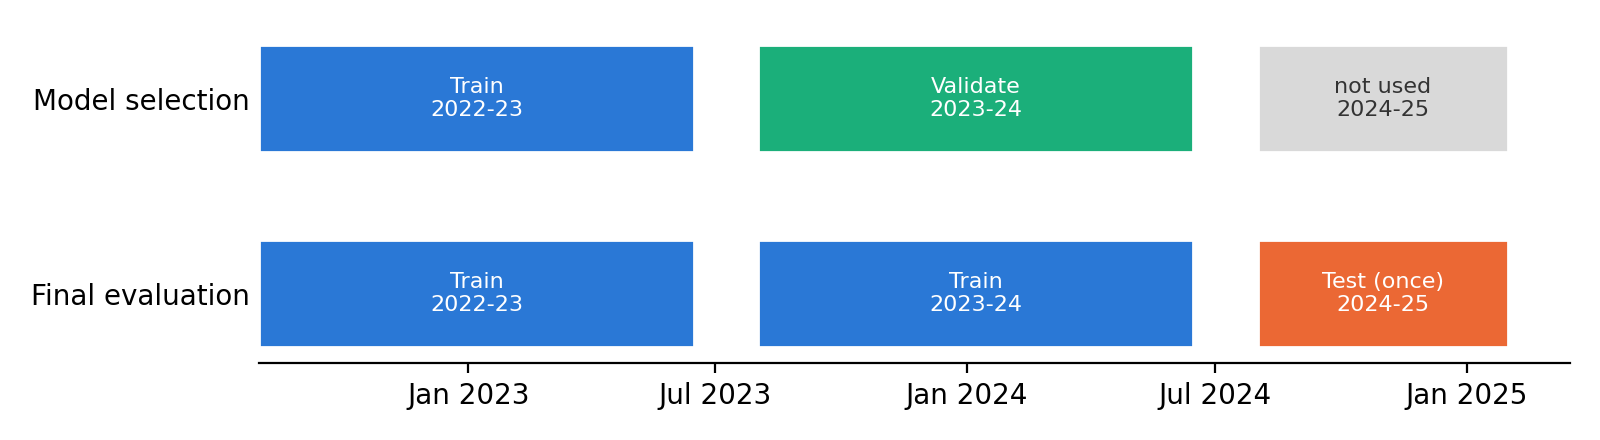
\includegraphics[width=\columnwidth]{figures/fig_split_timeline.png}
\caption{Forward-chaining validation design.}
\label{fig:split}
\end{figure}

The primary metric is the macro-F1 of T2 over all hours of the validation season, $\text{macro-F1}=\frac{1}{3}\sum_{k}\text{F1}_k$, which weights the rare congested class as much as the frequent free class. Secondary metrics are accuracy, per-class F1 and the confusion matrix for T2; MAE, RMSE and $R^2$ for T1; the area under the precision--recall curve (PR-AUC), which is more informative than ROC-AUC for rare events \cite{saito2015}, for T3; and, for the predicted probabilities, the Brier score \cite{brier1950}, the log loss and reliability curves \cite{niculescu2005}. Every metric is reported for all hours, for match windows ($-3$ to $+4$\,h at the stadium of the match) and for the post-match hours in the NEAR ring. The gain from the event features is tested with a bootstrap \cite{efron1993} that resamples whole matches, so that the correlated hours of a match stay together, and the importance of each feature group is measured by shuffling all of its columns together and recording the drop in macro-F1.

% =====================================================================
\section{Results}
\subsection{Match effects (RQ1, H1)}
Table~\ref{tab:h1} reports the effects in the NEAR ring with one observation per match. All nine stadium-by-window speed effects are negative and remain significant after Holm correction (\vHOneSpeedSigHolm of 9). In the pooled sample the speed change relative to the control days is \vPreDS, \vDuringDS and \vPostDS km/h before, during and after the match, and \vPostDV\,\% more vehicles are observed after it. Fig.~\ref{fig:obs} shows that the slowdown peaks in the hour after the final whistle and has largely disappeared five hours after kick-off. Before kick-off, \c{S}ükrü Saraco\u{g}lu and Tüpra\c{s} show slower traffic with about 16\,\% \emph{fewer} vehicles, consistent with closures and parking restrictions around these inner-city venues, whereas after the match Rams Park and \c{S}ükrü Saraco\u{g}lu show slower traffic with \emph{more} vehicles, the signature of departing spectators. The post-match distribution is skewed to the left (skewness \vPostSkew; median \vPostMedian km/h): a minority of matches produce very large slowdowns. The Shapiro--Wilk test rejected normality for \vShapiroShare\,\% of the speed distributions, so the rank-based tests are the main tests.

\begin{table}[t]
\caption{Match effects in the NEAR ring by stadium and window (H1)}
\label{tab:h1}
\centering\footnotesize
\fitcol{% generated by tools/build_paper.py - do not edit
\begin{tabular}{@{}llrccc@{}}
\toprule
Stadium & Window & $n$ & $\Delta$ speed, km/h [95\% CI] & $\Delta$ vehicles, \% [95\% CI] & $p_W$ \\
\midrule
Rams Park & pre & 60 & \ensuremath{-}3.26 [\ensuremath{-}4.61, \ensuremath{-}1.92] & \ensuremath{-}4.7 [\ensuremath{-}10.4, 1.4] & \ensuremath{<}0.001 \\
 & during & 60 & \ensuremath{-}5.70 [\ensuremath{-}6.56, \ensuremath{-}4.83] & 10.4 [5.5, 15.4] & \ensuremath{<}0.001 \\
 & post & 60 & \ensuremath{-}9.54 [\ensuremath{-}10.67, \ensuremath{-}8.41] & 26.5 [23.2, 29.8] & \ensuremath{<}0.001 \\
\midrule
{\c{S}}. Saraco{\u{g}}lu & pre & 58 & \ensuremath{-}3.88 [\ensuremath{-}4.27, \ensuremath{-}3.48] & \ensuremath{-}16.0 [\ensuremath{-}19.4, \ensuremath{-}12.4] & \ensuremath{<}0.001 \\
 & during & 57 & \ensuremath{-}2.26 [\ensuremath{-}2.66, \ensuremath{-}1.86] & \ensuremath{-}7.3 [\ensuremath{-}10.6, \ensuremath{-}3.9] & \ensuremath{<}0.001 \\
 & post & 60 & \ensuremath{-}4.41 [\ensuremath{-}4.86, \ensuremath{-}3.96] & 16.2 [11.8, 20.8] & \ensuremath{<}0.001 \\
\midrule
T{\"u}pra{\c{s}} & pre & 47 & \ensuremath{-}1.10 [\ensuremath{-}1.69, \ensuremath{-}0.52] & \ensuremath{-}16.1 [\ensuremath{-}19.9, \ensuremath{-}12.1] & \ensuremath{<}0.001 \\
 & during & 47 & \ensuremath{-}1.63 [\ensuremath{-}2.20, \ensuremath{-}1.06] & \ensuremath{-}14.9 [\ensuremath{-}19.4, \ensuremath{-}10.0] & \ensuremath{<}0.001 \\
 & post & 50 & \ensuremath{-}3.11 [\ensuremath{-}3.65, \ensuremath{-}2.57] & 0.5 [\ensuremath{-}3.8, 4.9] & \ensuremath{<}0.001 \\
\midrule
Pooled & pre & 165 & \ensuremath{-}2.86 [\ensuremath{-}3.42, \ensuremath{-}2.31] & \ensuremath{-}12.1 [\ensuremath{-}14.7, \ensuremath{-}9.3] & \ensuremath{<}0.001 \\
 & during & 164 & \ensuremath{-}3.34 [\ensuremath{-}3.81, \ensuremath{-}2.87] & \ensuremath{-}3.6 [\ensuremath{-}6.5, \ensuremath{-}0.6] & \ensuremath{<}0.001 \\
 & post & 170 & \ensuremath{-}5.84 [\ensuremath{-}6.45, \ensuremath{-}5.22] & 14.7 [11.9, 17.6] & \ensuremath{<}0.001 \\
\bottomrule
\end{tabular}}
\\[2pt]{\scriptsize $p_W$: Wilcoxon signed-rank test (speed); all speed effects keep $p<0.05$ after Holm correction.}
\end{table}

\begin{figure}[t]
\centering
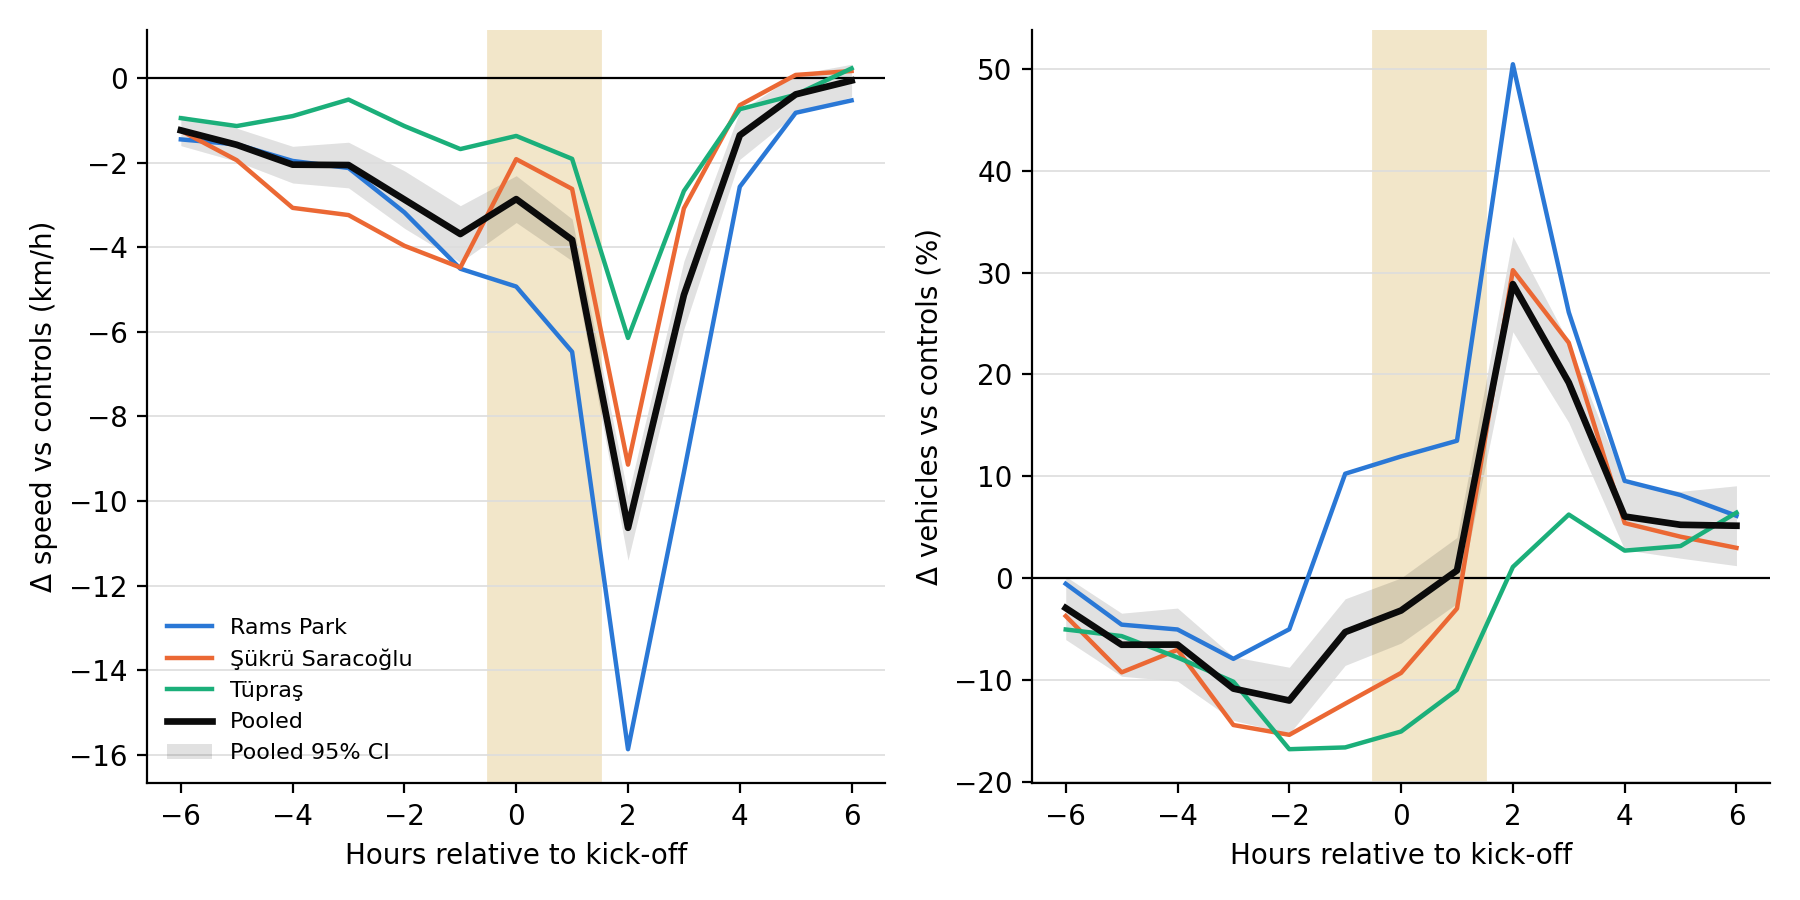
\includegraphics[width=\columnwidth]{figures/fig_event_study_observed.png}
\caption{Mean match effect by hour relative to kick-off: speed (left) and observed vehicles (right); band: 95\,\% CI of the pooled mean.}
\label{fig:obs}
\end{figure}

\subsection{Heterogeneity (RQ2, H2)}
Table~\ref{tab:h2} lists the comparisons of the post-match effect. The stadium is by far the most important factor: it explains $\eta^2=\vStEta$ of the variance, and the slowdown at Rams Park (\vPostRams km/h) is about twice that at \c{S}ükrü Saraco\u{g}lu (\vPostSaracoglu) and three times that at Tüpra\c{s} (\vPostTupras). Big matches show a somewhat larger slowdown (\vBigMean vs \vBigOther km/h, $n=\vBigN$; t-test $p=\vBigP$, Mann--Whitney $p=\vBigPU$), but the difference does not survive Holm correction ($p=\vBigPHolm$). Istanbul opponents, which bring few travelling fans, do not differ from other domestic opponents (\vIstMean vs \vIstOther km/h, $p=\vIstP$), and the opponent group as a whole explains almost nothing (ANOVA $p=\vOppAnovaP$, Kruskal--Wallis $p=\vOppKwP$, $\eta^2=\vOppEta$; Fig.~\ref{fig:opp}). Derby status, weekday, weather and kick-off slot show no significant differences, and none of the attributes is correlated with the size of the effect. Domestic-cup matches are followed by smaller slowdowns than league matches, but the competition factor as a whole is not significant after correction (Kruskal--Wallis Holm $p=\vCompKwPHolm$). Overall, \vHTwoSigRaw of \vHTwoTests rank-based tests are significant before and \vHTwoSigHolm after Holm correction, and all survivors concern the stadium or the league--cup contrast. Small groups (14 derbies, 5 afternoon matches) limit the power of some comparisons.

\begin{table*}[t]
\caption{Post-match effect by match attributes, NEAR ring (H2)}
\label{tab:h2}
\centering\footnotesize
\begin{adjustbox}{max width=\textwidth}% generated by tools/build_paper.py - do not edit
\begin{tabular}{@{}lcrrrr@{}}
\toprule
 & Group means, km/h ($n$) & \multicolumn{2}{c}{Raw $p$} & \multicolumn{2}{c}{Holm $p$} \\
\cmidrule(lr){3-4}\cmidrule(lr){5-6}
Comparison & or effect size & param. & rank & param. & rank \\
\midrule
Derby vs other & \ensuremath{-}7.38 (14) vs \ensuremath{-}5.70 (156) & 0.140 & 0.402 & 1.000 & 1.000 \\
Big match vs other & \ensuremath{-}7.64 (18) vs \ensuremath{-}5.62 (152) & 0.047 & 0.209 & 0.746 & 1.000 \\
Istanbul vs other domestic opponent & \ensuremath{-}5.60 (37) vs \ensuremath{-}5.72 (78) & 0.876 & 0.886 & 1.000 & 1.000 \\
Opponent group (4 groups) & $\eta^2$ = 0.024 & 0.255 & 0.657 & 1.000 & 1.000 \\
Weekend vs weekday & \ensuremath{-}6.35 (77) vs \ensuremath{-}5.41 (93) & 0.137 & 0.216 & 1.000 & 1.000 \\
Wet vs dry & \ensuremath{-}6.12 (27) vs \ensuremath{-}5.79 (143) & 0.701 & 0.969 & 1.000 & 1.000 \\
Kick-off slot (3 groups) & $\eta^2 < 0.001$ & 0.966 & 0.814 & 1.000 & 1.000 \\
Competition (3 groups) & $\eta^2$ = 0.048 & 0.016 & 0.004 & 0.276 & 0.073 \\
League vs domestic cup & \ensuremath{-}6.30 (118) vs \ensuremath{-}3.20 (15) & \ensuremath{<}0.001 & \ensuremath{<}0.001 & \ensuremath{<}0.001 & 0.016 \\
Stadium (3 groups) & $\eta^2$ = 0.470 & \ensuremath{<}0.001 & \ensuremath{<}0.001 & \ensuremath{<}0.001 & \ensuremath{<}0.001 \\
\bottomrule
\end{tabular}\end{adjustbox}
\\[2pt]{\scriptsize param.: t-test (two groups) or ANOVA; rank: Mann--Whitney U or Kruskal--Wallis.}
\end{table*}

\begin{figure}[t]
\centering
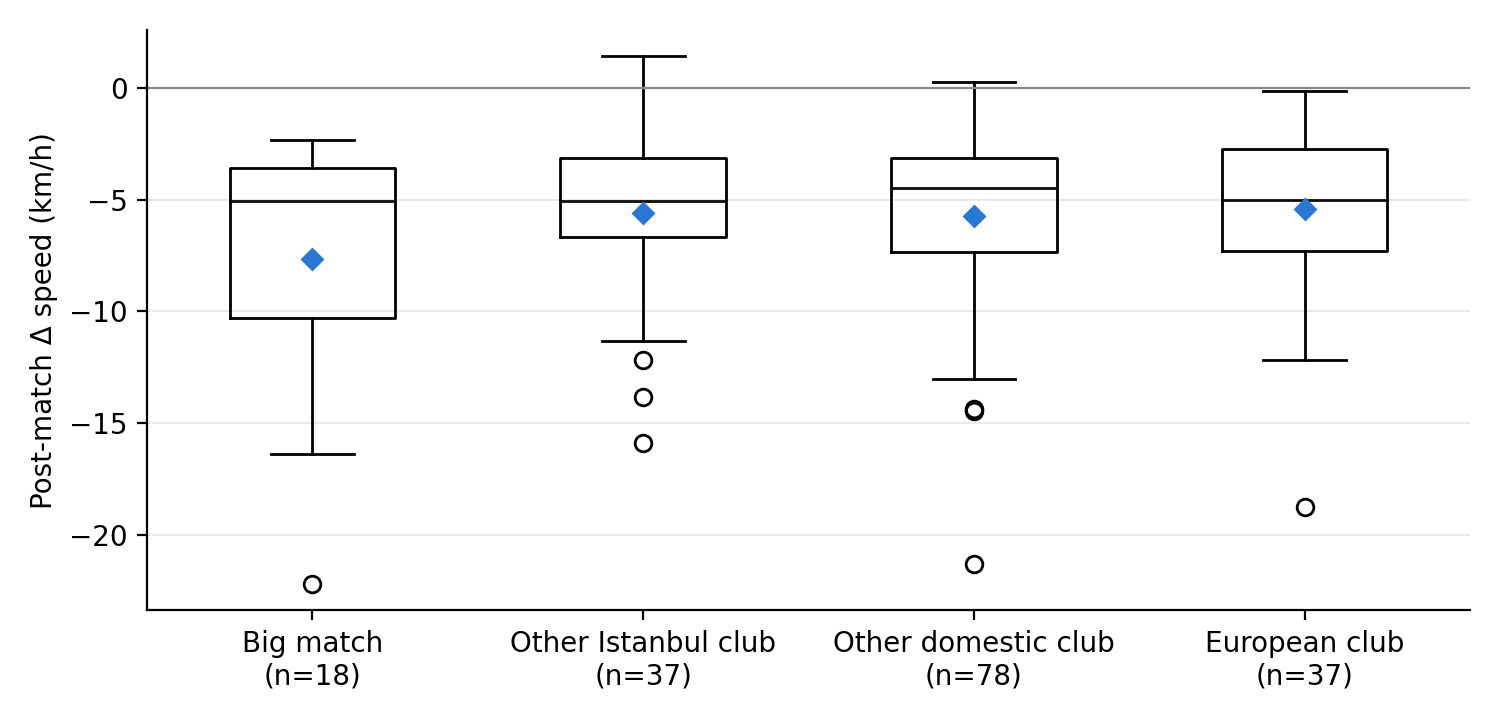
\includegraphics[width=0.9\columnwidth]{figures/fig_opponent_groups.png}
\caption{Post-match speed effect in the NEAR ring by opponent group (diamond: mean).}
\label{fig:opp}
\end{figure}

\subsection{Robustness (H3, H4)}
All falsification checks behave as expected for a genuine match effect (Table~\ref{tab:robust}). Pseudo-events on non-match days (\vPlacebo km/h, $p=\vPlaceboP$) and matches of the closed-doors season (\vClosedDoors km/h, $p=\vClosedDoorsP$) show no significant change, which links the slowdown to the spectators. Subtracting the change in the distal ring gives \vDiD km/h, close to the NEAR estimate, so city-wide differences between match and control days explain little of the effect. The effect decays with distance from \vRingZero km/h in R0 to \vRingOne in R1 and \vRingTwo in R2. Excluding the \vPctRelaxed\,\% of matches whose weather rule was relaxed leaves \vSensMean km/h \vSensCI ($n=\vSensN$), practically the main estimate. In the evening hours of the NEAR cells, the congested class is more frequent in match windows than outside them (\vCongWin\,\% vs \vCongOther\,\%; $\chi^2=\vChiSq$, $p<0.001$), but Cramér's $V=\vCramerV$ shows that the association is small compared with the overall variability of traffic---a first hint that match information matters mainly inside the match windows.

\begin{table}[t]
\caption{Robustness and sensitivity checks, post-match window}
\label{tab:robust}
\centering\footnotesize
\fitcol{% generated by tools/build_paper.py - do not edit
\begin{tabular}{@{}lrrcrr@{}}
\toprule
Check (post-match window) & $n$ & Mean & 95\% CI & $p_t$ & $p_W$ \\
\midrule
Placebo dates (pseudo-events) & 136 & \ensuremath{-}0.23 & [\ensuremath{-}0.56, 0.11] & 0.189 & 0.953 \\
Closed-doors season 2020-21 & 62 & 0.16 & [\ensuremath{-}0.55, 0.88] & 0.648 & 0.549 \\
Difference-in-differences, NEAR $-$ distal & 170 & \ensuremath{-}5.12 & [\ensuremath{-}5.71, \ensuremath{-}4.54] & \ensuremath{<}0.001 & \ensuremath{<}0.001 \\
Spatial decay R0 $-$ R1 & 170 & \ensuremath{-}4.12 & [\ensuremath{-}4.80, \ensuremath{-}3.44] & \ensuremath{<}0.001 & \ensuremath{<}0.001 \\
Spatial decay R1 $-$ R2 & 170 & \ensuremath{-}2.86 & [\ensuremath{-}3.13, \ensuremath{-}2.58] & \ensuremath{<}0.001 & \ensuremath{<}0.001 \\
Strict weather matching only & 110 & \ensuremath{-}5.88 & [\ensuremath{-}6.66, \ensuremath{-}5.09] & \ensuremath{<}0.001 & \ensuremath{<}0.001 \\
\bottomrule
\end{tabular}}
\end{table}

\subsection{External validation with two further open sources}
\label{sec:external}
\textit{Rail stations.} With the matched-control design of Eq.~\eqref{eq:delta} applied to daily data (same weekday 1--4 weeks away, no home match of the three clubs, no holiday; one value per match), station entries on match days exceed those of the control days by \vExtRailMean\,\% on average (median \vExtRailMedian\,\%, 95\,\% CI \vExtRailCI, $n=\vExtRailN$ matches with spectators, Wilcoxon $p<0.001$): \vExtRailRams\,\% at Seyrantepe, which serves little other demand, \vExtRailSar\,\% at Sö\u{g}ütlüçe\c{s}me and \vExtRailTup\,\% at Kabata\c{s} (Fig.~\ref{fig:rail}). The increase is the same in the traffic study period (\vExtRailStudy\,\%, $n=\vExtRailStudyN$) and after the traffic data end (February to December 2025: \vExtRailAfter\,\% \vExtRailAfterCI, $n=\vExtRailAfterN$), whereas closed-doors matches show no increase (median \vExtRailClosedMed\,\%, $p=\vExtRailClosedP$, $n=\vExtRailClosedN$; the weekend curfews of early 2021 lower the mean). The two sources agree at match level: the larger the increase in station entries, the larger the post-match slowdown of the same match measured with the traffic data (Spearman $\rho=\vExtLinkRho$, $n=\vExtLinkN$, $p<0.001$).

\textit{Traffic announcements.} UYM announced road closures or congestion caused by the match for \vExtUymWith of the \vExtUymMatches matches with spectators (\vExtUymShare\,\%), including \vExtUymAfterWith matches after January 2025, and for none of the \vExtUymClosedMatches closed-doors matches. Of these announcements, \vExtUymClosure\,\% are road closures and \vExtUymBefore\,\% start before kick-off (median \vExtUymMedianH\,h before), which supports reading the pre-match slowdown with fewer vehicles at \c{S}ükrü Saraco\u{g}lu and Tüpra\c{s} as an effect of closures. Ordinary incident announcements (accidents, breakdowns and congestion not linked to the match) within 2\,km of the stadium do not rise clearly in the match window (rate ratio \vExtIncRR, 95\,\% bootstrap CI \vExtIncCI).

\begin{figure}[t]
\centering
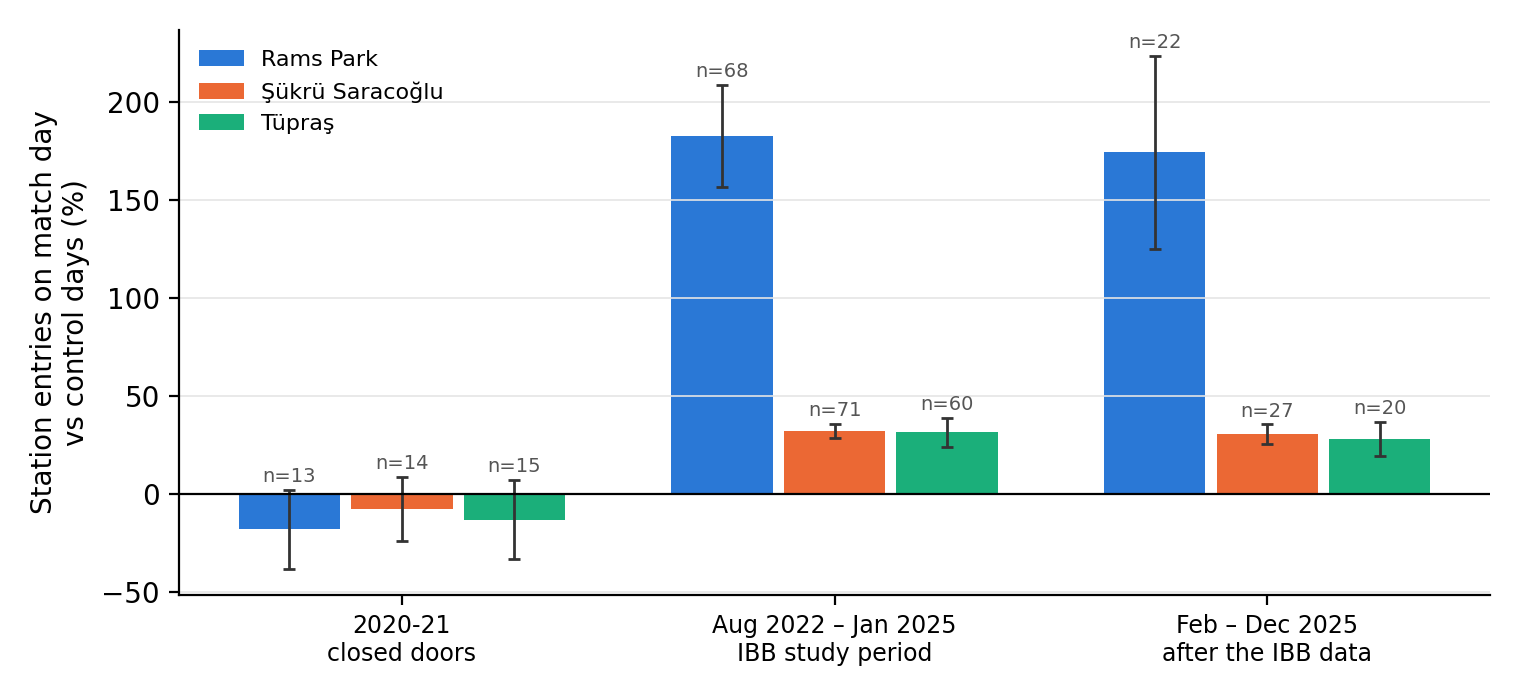
\includegraphics[width=\columnwidth]{figures/fig_extra_rail.png}
\caption{Entries at the rail stations next to the stadiums on match days relative to matched control days (mean and 95\,\% CI), by period.}
\label{fig:rail}
\end{figure}

\subsection{Model selection}
Table~\ref{tab:select} shows the validation season. Gradient boosting reaches the highest macro-F1, clearly ahead of logistic regression and the profile baseline; the random forest comes close to the gradient-boosting settings. The setting with \vBestLeaves leaves and no class weights was selected; balanced class weights would raise the F1 of the congested class at a small cost in overall macro-F1, a trade-off discussed in Section~\ref{sec:discussion}.

\begin{table}[t]
\caption{Model selection on the validation season (T2)}
\label{tab:select}
\centering\footnotesize
\fitcol{% generated by tools/build_paper.py - do not edit
\begin{tabular}{@{}lccc@{}}
\toprule
Model (validation season 2023-24) & macro-F1, all & macro-F1, match & F1 congested \\
\midrule
Gradient boosting, 31 leaves, weights: none & 0.763 & 0.689 & 0.612 \\
Gradient boosting, 63 leaves, weights: none & 0.762 & 0.699 & 0.611 \\
Gradient boosting, 31 leaves, weights: balanced & 0.757 & 0.696 & 0.628 \\
Gradient boosting, 63 leaves, weights: balanced & 0.760 & 0.706 & 0.635 \\
Logistic regression & 0.734 & 0.594 & 0.596 \\
Random forest & 0.758 & 0.667 & 0.633 \\
Baseline: hour-of-week profile & 0.726 & 0.609 & 0.540 \\
\bottomrule
\end{tabular}}
\end{table}

\subsection{Test-season performance (RQ3, H5)}
Table~\ref{tab:models} and Fig.~\ref{fig:compare} report the single evaluation on the 2024-25 season. Gradient boosting with all features is the best model on almost every metric: macro-F1 \vFOneHgbAll over all hours (baselines \vFOneBZeroAll and \vFOneBOneAll, logistic regression \vFOneLinAll, random forest \vFOneRfAll) and an MAE of \vMaeHgbAll km/h with $R^2=\vRTwoHgbAll$ for speed. The ranking---boosting ahead of the random forest ahead of the linear model---shows that the relationships are strongly non-linear: a match effect is an interaction of ``match day'', ``two hours after kick-off'' and ``this stadium'', which trees represent naturally and a linear model does not.

\begin{table*}[t]
\caption{Test-season results (2024-25); best value per column in bold}
\label{tab:models}
\centering\footnotesize
\begin{adjustbox}{max width=\textwidth}% generated by tools/build_paper.py - do not edit
\begin{tabular}{@{}lcccccccc@{}}
\toprule
 & \multicolumn{3}{c}{T2 congestion class} & \multicolumn{3}{c}{T1 average speed, MAE (km/h)} & \multicolumn{2}{c}{T3 abnormal slowdown} \\
\cmidrule(lr){2-4}\cmidrule(lr){5-7}\cmidrule(lr){8-9}
 & macro-F1 & macro-F1 & F1 congested & all & match & post-match & PR-AUC & PR-AUC \\
Model & all hours & match windows & post, NEAR & hours & windows & NEAR & all hours & match windows \\
\midrule
Baseline: same hour last week & 0.742 & 0.613 & 0.133 & 3.09 & 4.74 & 7.18 & 0.072 & 0.142 \\
Baseline: hour-of-week profile & 0.746 & 0.607 & 0.064 & 2.84 & 4.31 & 6.80 & -- & -- \\
Logistic / ridge regression & 0.751 & 0.597 & \textbf{0.555} & 2.60 & 3.97 & 5.25 & 0.105 & 0.280 \\
Random forest & 0.779 & 0.663 & 0.510 & 2.46 & 3.64 & 5.44 & -- & -- \\
Gradient boosting, no match features & 0.794 & 0.633 & 0.038 & 2.41 & 4.07 & 6.68 & 0.088 & 0.196 \\
Gradient boosting, all features & \textbf{0.797} & \textbf{0.702} & 0.533 & \textbf{2.38} & \textbf{3.12} & \textbf{3.68} & \textbf{0.147} & \textbf{0.501} \\
\bottomrule
\end{tabular}\end{adjustbox}
\\[2pt]{\scriptsize Match windows: $-3$ to $+4$\,h relative to kick-off at the stadium of the match. Post, NEAR: $+2$ to $+4$\,h in R0 and R1. T3 decision thresholds were chosen on the validation season.}
\end{table*}

\begin{figure}[t]
\centering
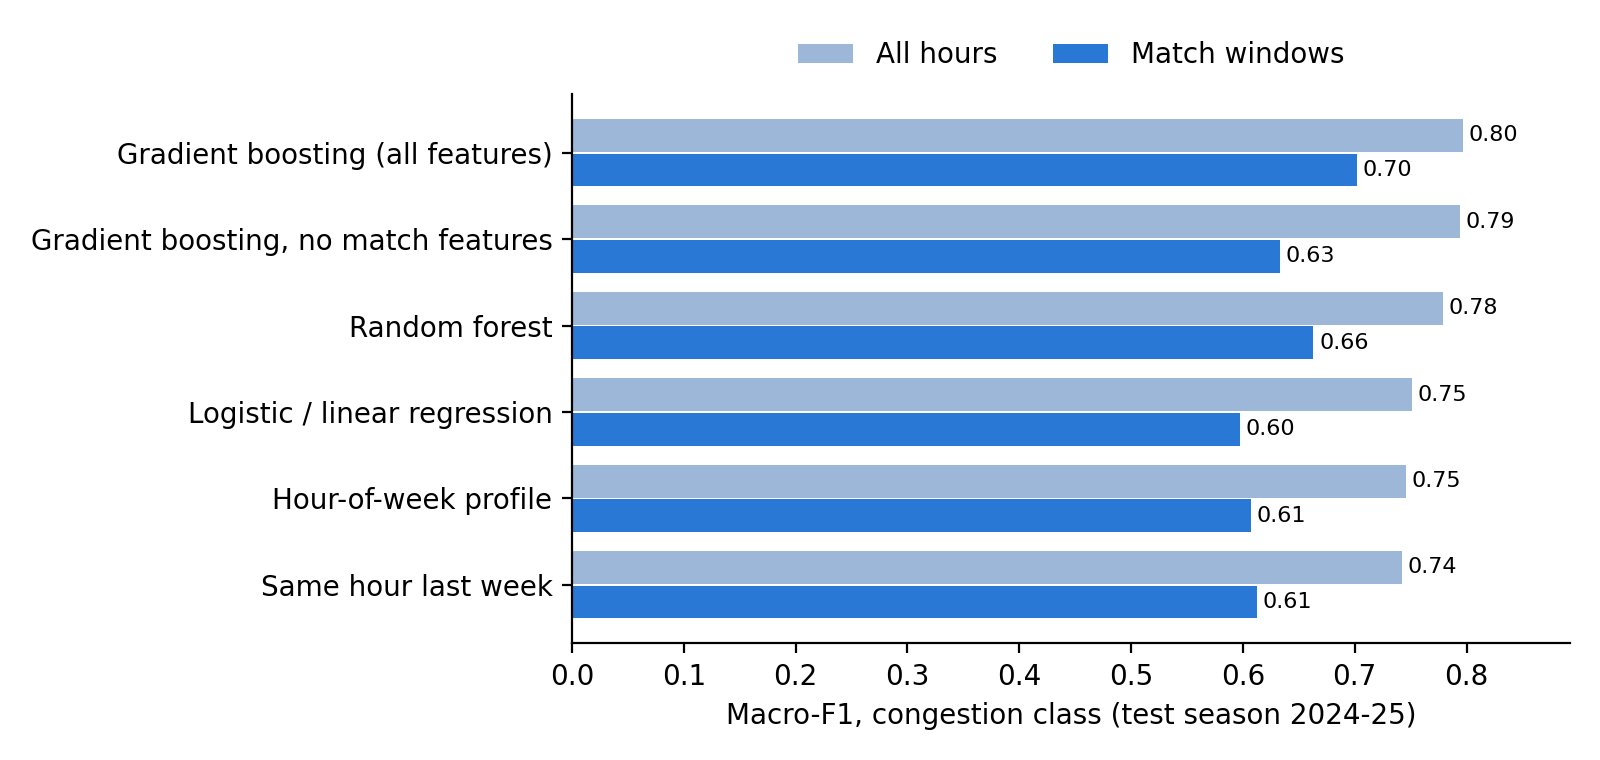
\includegraphics[width=\columnwidth]{figures/fig_model_comparison.png}
\caption{Macro-F1 of the congestion class on the test season, over all hours and in match windows.}
\label{fig:compare}
\end{figure}

The value of fixture information depends entirely on \emph{when} it is measured. Over all hours, removing the event features changes macro-F1 only from \vFOneHgbAll to \vFOneNoEvAll, because matches affect a few percent of the hours. In the match windows, however, macro-F1 falls from \vFOneHgbMatch to \vFOneNoEvMatch, and in the post-match hours near the stadiums the speed error grows from \vMaeHgbPost to \vMaeNoEvPost km/h and the F1 of the congested class collapses from \vFCongHgbPost to \vFCongNoEvPost. Fig.~\ref{fig:pred} makes the mechanism visible: the model without fixture information predicts an ordinary evening (\vPeakNoEv km/h two hours after kick-off), while the full model follows the observed dip (\vPeakHgb vs \vPeakObs km/h). In the post-match hours the congested class is observed in \vPostCongObs\,\% of the NEAR cell-hours and predicted in \vPostCongHgb\,\% by the full model but only \vPostCongNoEv\,\% without fixture features. The bootstrap over the \vBootMatches test matches with observed match windows confirms the gain: the fixture features reduce the MAE in match windows by \vBootMae km/h \vBootMaeCI and raise macro-F1 by \vBootFOne \vBootFOneCI; all bootstrap samples favour the full model, so H5 is rejected. For the rare abnormal slowdown (T3), the full model raises PR-AUC in match windows from \vPrNoEvMatch to \vPrHgbMatch.

\begin{figure}[t]
\centering
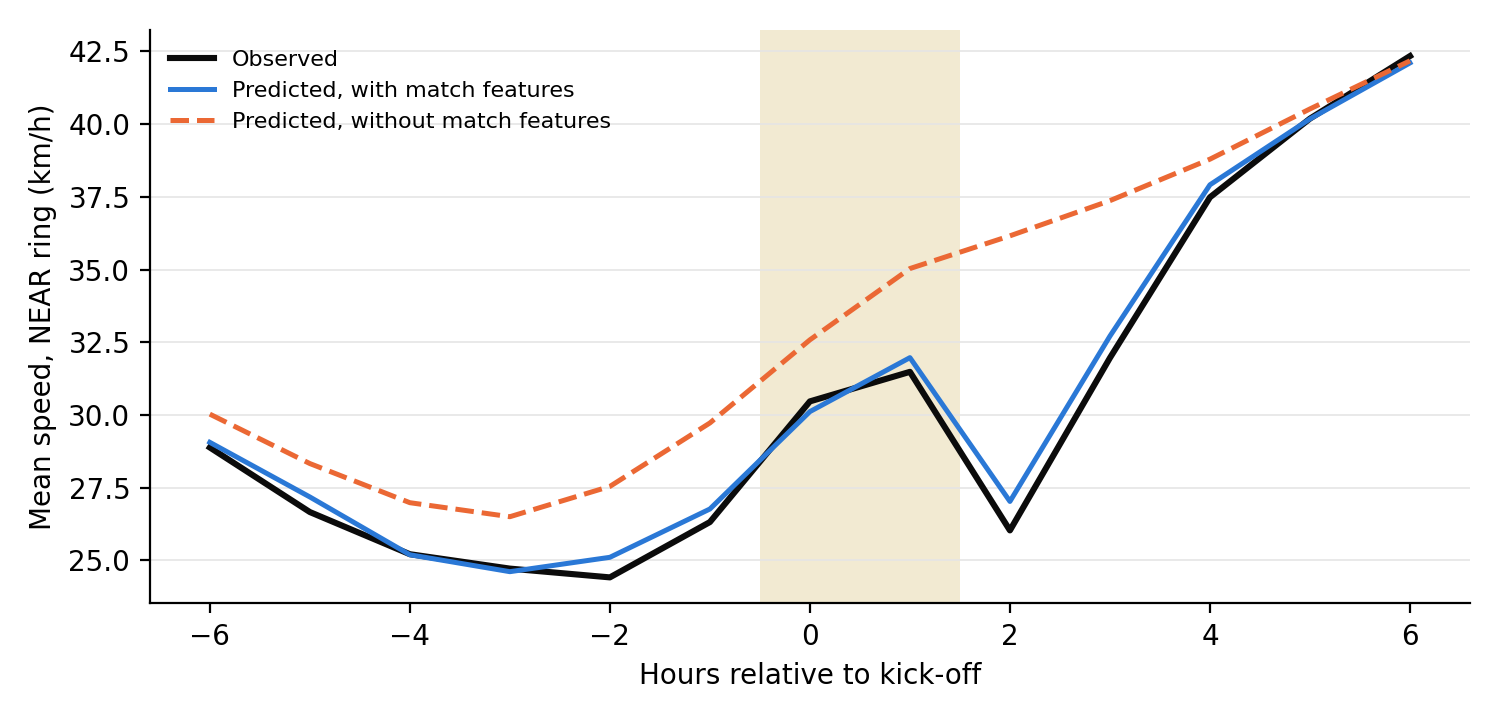
\includegraphics[width=\columnwidth]{figures/fig_event_study_predicted.png}
\caption{Observed and day-ahead predicted speed in the NEAR ring around the 2024-25 test matches, with and without fixture features (shaded: during window).}
\label{fig:pred}
\end{figure}

\subsection{Feature importance, error analysis and calibration}
\label{sec:importance}
Fig.~\ref{fig:importance} shows the drop in macro-F1 when a feature group is shuffled. Traffic history dominates everywhere (\vImpHistoryAll over all hours, \vImpHistoryMatch in match windows). The event group is almost irrelevant over all hours (\vImpEventAll) but becomes the second most important group in match windows (\vImpEventMatch). Weather matters least (\vImpWeatherAll), in line with the absence of weather differences in H2; this also means that replacing reanalysis by forecast weather would change little.

\begin{figure}[t]
\centering
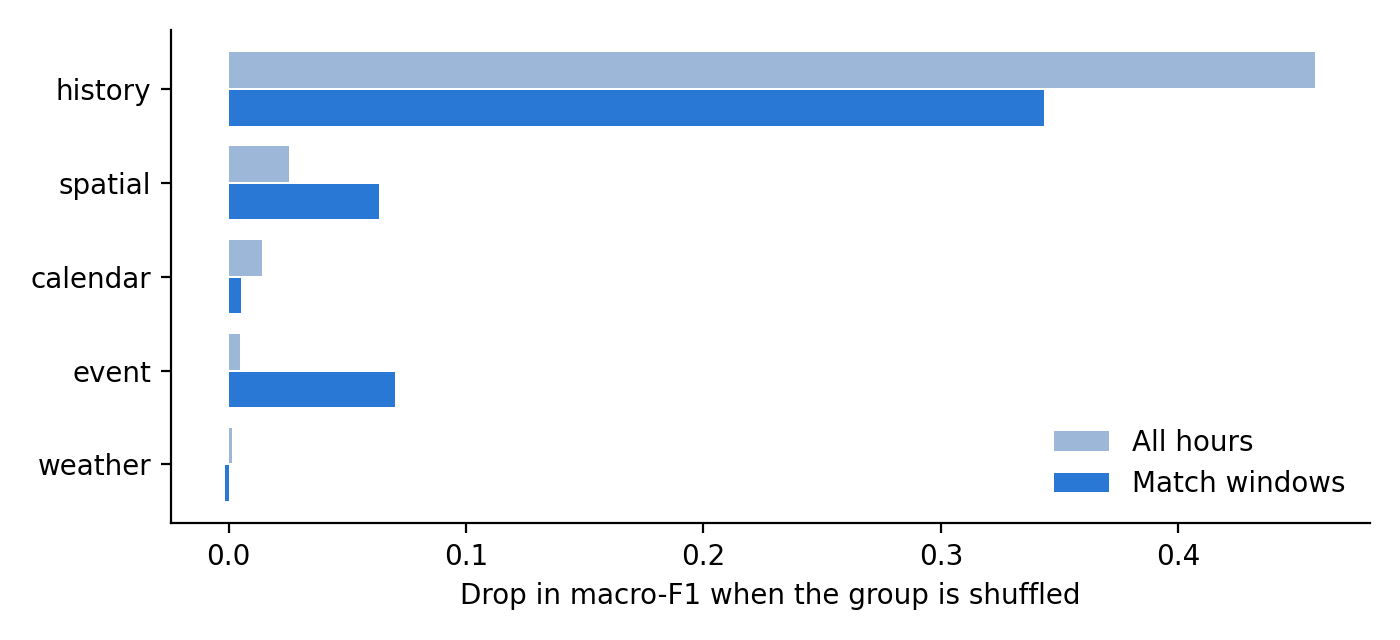
\includegraphics[width=\columnwidth]{figures/fig_group_importance.png}
\caption{Group permutation importance of the gradient-boosting model (T2, test season).}
\label{fig:importance}
\end{figure}

Table~\ref{tab:error} breaks the speed error down by stadium and window. Fixture features never hurt: outside match windows both models have the same error, while in the post-match window the error at Rams Park falls from about 8 to under 5\,km/h. The largest remaining errors occur at Rams Park, the stadium with the largest and most variable effect, and the full model still slightly underestimates the post-match slowdown there. In the match windows, the confusion matrix shows that \vCongRecall\,\% of the congested hours are recognised and \vCongAsModerate\,\% are predicted as moderate; free and moderate hours are recognised in \vFreeRecall\,\% and \vModRecall\,\% of the cases (Fig.~\ref{fig:confusion}). Errors between neighbouring classes are therefore far more common than confusions of free and congested traffic.

\begin{table}[t]
\caption{Speed MAE (km/h) by stadium and window, test season: with / without fixture features}
\label{tab:error}
\centering\footnotesize
\fitcol{% generated by tools/build_paper.py - do not edit
\begin{tabular}{@{}lcccc@{}}
\toprule
Stadium & pre & during & post & no match \\
\midrule
Rams Park & 4.17 / 5.27 & 3.69 / 4.28 & 4.61 / 8.07 & 3.01 / 3.02 \\
{\c{S}}. Saraco{\u{g}}lu & 2.71 / 3.27 & 2.63 / 2.85 & 3.11 / 3.74 & 2.19 / 2.20 \\
T{\"u}pra{\c{s}} & 2.01 / 2.28 & 1.91 / 2.12 & 2.13 / 2.62 & 1.81 / 1.81 \\
\bottomrule
\end{tabular}}
\end{table}

\begin{figure}[t]
\centering
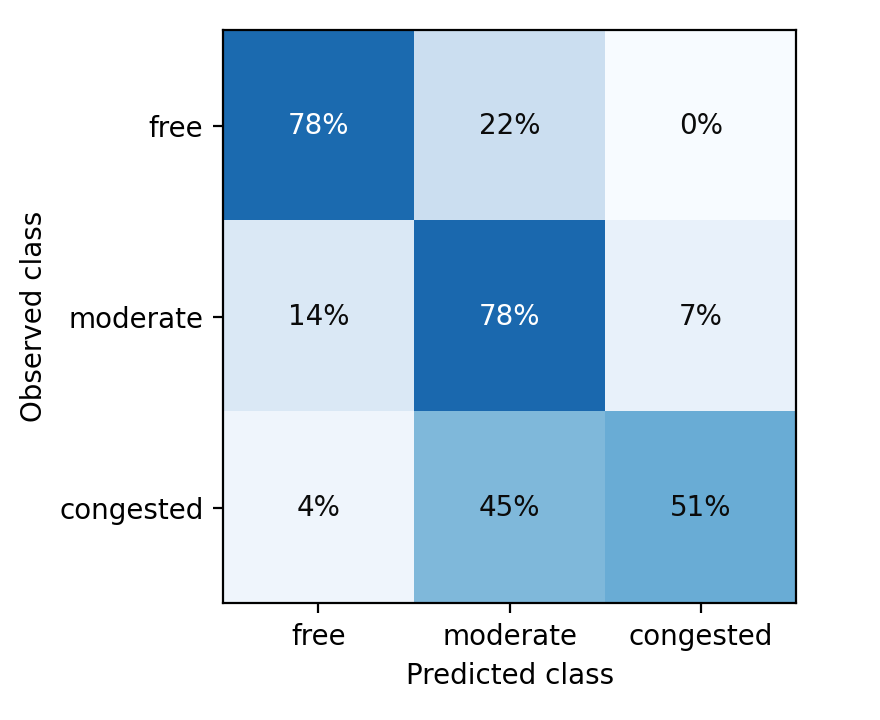
\includegraphics[width=0.58\columnwidth]{figures/fig_confusion_match.png}
\caption{Confusion matrix of the gradient-boosting model in the match windows of the test season (row-normalised, \%).}
\label{fig:confusion}
\end{figure}

The predicted probabilities of gradient boosting are well calibrated (Fig.~\ref{fig:calibration}). For T2, the multiclass Brier score is \vBrierTTwo against \vBrierTTwoRef for a constant class-frequency forecast, and the log loss is \vLogLossTTwo. For T3, the Brier score is \vBrierHgb against \vBrierRef for the constant prevalence forecast; the mean predicted probability (\vTThreeMeanPred\,\%) is slightly below the observed prevalence (\vTThreePrevTest\,\%). The logistic regression with balanced class weights, in contrast, has a Brier score of \vBrierLin: balancing improves the recall of rare classes but inflates the probabilities.

\begin{figure}[t]
\centering
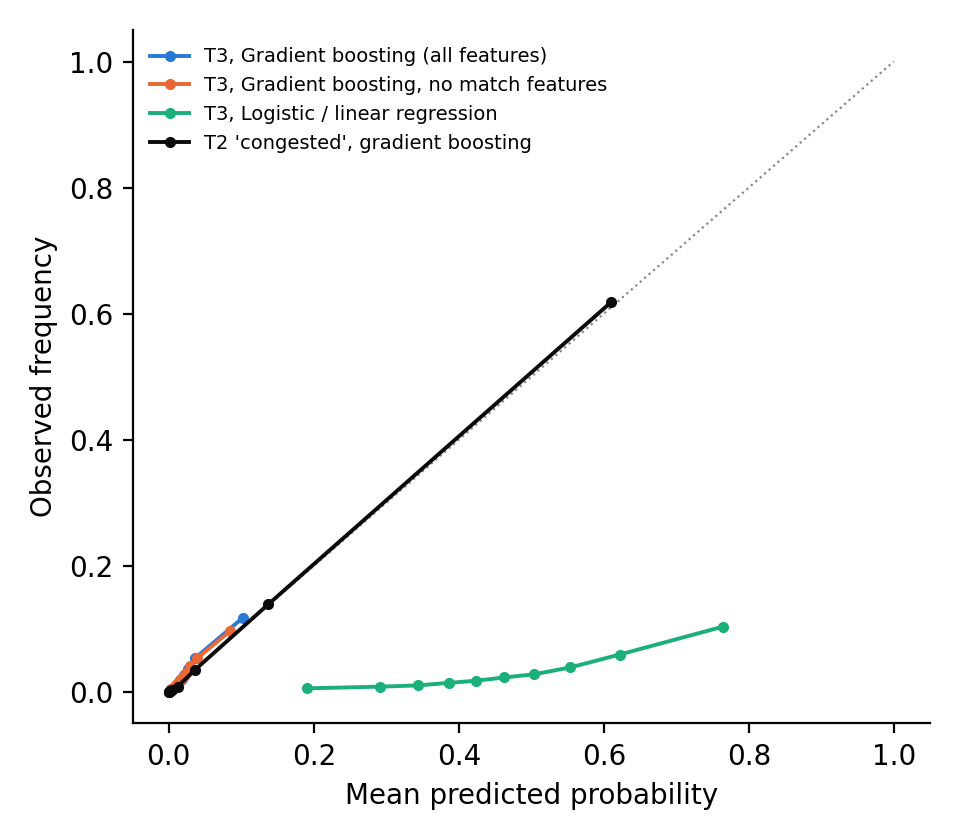
\includegraphics[width=0.68\columnwidth]{figures/fig_calibration.png}
\caption{Reliability curves on the test season (deciles of the predicted probability).}
\label{fig:calibration}
\end{figure}

\subsection{Comparison with the literature}
No published study predicts congestion classes around Istanbul stadiums, so no directly comparable score exists and the seasonal baselines serve as the reference point. Qualitatively, our findings agree with earlier work. As at the Los Angeles Coliseum \cite{giuliano2021}, a tree ensemble outperforms regression. Like Rodrigues \textit{et al.} \cite{rodrigues2019}, we find that event information reduces forecasting errors specifically in event areas and periods. The local effect we measure (about 15\,\% lower speed near the stadium after the match) is much larger than the city-wide 1.3\,\% increase in travel times reported for Yankee Stadium \cite{hwang2025}, which is consistent with that study's finding that effects concentrate near the venue. The dominant role of traffic history agrees with Özdenizci Köse \textit{et al.} \cite{ozdenizci2025}, who found traffic-specific variables to be the strongest predictors of Istanbul traffic density, and with the strong daily and weekly cycles described by \c{S}ahin and Çolako\u{g}lu \cite{sahin2025}; unlike in their city-wide setting, weather adds little to our day-ahead model once the traffic history is known.

% =====================================================================
\section{Discussion}
\label{sec:discussion}
\textit{What the results mean.} Football matches create a short, local and highly predictable disruption: speeds drop by about 15\,\% in the stadium cell and its neighbours, mostly in the hour after the final whistle, and the effect weakens strongly within about 2\,km. Which stadium hosts the match matters far more than who the opponent is or when the match starts. That the venue matters more than the attractiveness of a match suggests that the access network and the travel behaviour of the spectators drive the effect; one possible explanation for the large effect at Rams Park, which lies outside the dense centre, is a higher share of spectators travelling by car, but testing this requires modal-split data. Because fixtures are known weeks in advance, these disruptions can be forecast: a day-ahead model that knows the fixture almost halves the post-match speed error and recognises congested post-match hours that a model without fixture information almost never predicts.

\textit{Strengths.} The study uses open data only and can be rebuilt with one command. The counterfactual is explicit and checked with placebo dates, a closed-doors season, a distal reference ring and spatial decay. Inference uses one observation per match and is corrected for multiple testing. The prediction study is leakage-controlled (day-ahead features, baselines fitted on the training period, forward-chaining validation, a single test) and isolates the value of fixture information with an ablation and a match-level bootstrap. Two independent open sources, rail-station entries and control-centre announcements, confirm the crowd effect, the role of closures and the persistence of the effect after the traffic data end.

\textit{Weaknesses and sources of error.} Geohash cells are coarse and mix road types, so localised jams are diluted. The vehicle count is a sample whose coverage may change over time. Hourly resolution and kick-off rounding blur the window boundaries. Reanalysis weather is used instead of archived forecasts, which makes the day-ahead setting slightly optimistic, although weather proved to be the least important group. The test season covers only six months and \vTestMatches matches. The abnormal-slowdown target is defined relative to a historical baseline and is affected by drift: with the 2022-23 baseline its prevalence rose from \vTThreePrevSelTrain\,\% to \vTThreePrevSelVal\,\% in the next season. The model was selected for overall macro-F1, which slightly favours the frequent classes; an operator who cares mainly about congestion would choose balanced class weights at the cost of calibration. The traffic series ends in January 2025, so later seasons are covered only by the two indirect sources. Finally, the statistical design is observational and cannot prove causality, and the closed-doors season was also affected by pandemic restrictions.

\textit{Possible improvements.} Archived weather forecasts, road-segment probe data and hourly public-transport ridership would sharpen both parts of the study. Further venues and events (Ba\c{s}ak\c{s}ehir, concerts, basketball) would increase the number of matches and the power of the group comparisons. Rolling retraining would address drift, isotonic calibration could combine balanced weights with reliable probabilities, and graph-based models \cite{olug2024} could exploit the spatial propagation of congestion.

% =====================================================================
\section{Conclusion}
Football matches leave a clear, local and predictable trace in Istanbul's open traffic data. After a match, speed near the stadium is about 15\,\% lower than on comparable days, most of all at Rams Park; the effect is robust to placebo, closed-doors, distal-ring and multiple-testing checks and does not depend on the opponent, kick-off time or weather. A leakage-controlled day-ahead gradient-boosting model predicts the congestion class better than seasonal baselines, linear models and random forests, and fixture information is what allows it to anticipate post-match congestion. Rail-station entries and traffic-control announcements confirm the effect independently and show that it continues after January 2025. Open municipal data and published fixtures are thus sufficient to quantify and forecast the traffic cost of large planned events, a result that can support match-day traffic management and can be extended to other venues and event types.

\section*{Use of Generative AI}
A generative AI assistant (Claude, Anthropic) was used as a supporting tool for code development and debugging, for checking statistical procedures and for language editing. All analyses were run by the authors on the data described above, every number in this paper is produced by the accompanying code, and the authors verified the results and references and can explain every step.

\bibliographystyle{IEEEtran}
\bibliography{references}

\end{document}
